\documentclass{article}

\usepackage{minitoc}
\usepackage{tabularx}
\usepackage{booktabs}
\usepackage{graphicx}
\usepackage{hyperref}
\usepackage{xcolor}
\usepackage{blkarray}
\usepackage{amsthm, amssymb, amsmath}
\usepackage{caption}
\usepackage{subcaption}
\usepackage{multirow}
\usepackage[ruled,vlined]{algorithm2e}

\usepackage{natbib}
\bibliographystyle{abbrvnat}

\theoremstyle{definition}
\newtheorem{definition}{Definition}[section]
\newtheorem{theorem}{Theorem}[section]
\newtheorem{lemma}[theorem]{Lemma}
\newtheorem{conjecture}[theorem]{Conjecture}
\newtheorem{Prop}{Proposition}

\usepackage[margin=2.5cm, includefoot, footskip=30pt]{geometry}
\pagestyle{plain}
\setlength{\parindent}{0em}
\setlength{\parskip}{1em}

\renewcommand{\baselinestretch}{1}

\usepackage{standalone}

\newtheorem{proposition}{Proposition}

\title{Reactive strategies with longer memory}

\author{Nikoleta E. Glynatsi, Ethan Akin, Martin Nowak, Christian Hilbe}
\date{}

\begin{document}

\maketitle

\section{Formal Model}

We consider infinitely repeated games among two players, player $p$ and
player $q$. Each round, they engage in the donation game with payoff matrix

\begin{equation} \label{Eq:DonationGame}
\left(
\begin{array}{cc}
b-c	&-c\\
b	&0
\end{array}
\right).
\end{equation}

Here $b$ and $c$ denote the benefit and the cost of cooperation, respectively. 
We assume $b\!>\!c\!>\!0$ throughout.
Therefore, the payoff matrix~\eqref{Eq:DonationGame} is a special case of the
prisoner's dilemma with payoff matrix,

\begin{equation} \label{Eq:PrisonerDilemma}
    \left(
    \begin{array}{cc}
    R & S\\
    T & P
    \end{array}
    \right),
\end{equation}

with $T > R > S > P$ and $2 R > T + S$. Here, $R$ is the reward payoff of mutual
cooperation, $T$ is the temptation to defect payoff, $S$ is the sucker's payoff,
and $P$ is the punishment payoff for mutual defection.

We assume in the following, that the players' decisions only depend on the
outcome of the previous $n$ rounds. To this end, an {\it $n$-history for player
$p$} is a string $h^p=(a^p_{-1},\ldots,a^p_{-n})\!\in\!\{C,D\}^n$. An entry
$a^p_{-k}$ corresponds to player $p$'s action $k$ rounds ago. Let $H^p$ denote
the space of all $n$-histories of player~$p$. Analogously, we define $H^q$ as
the set of $n$-histories $h^q$ of player~$q$. Sets $H^p$ and $H^q$ contain
$|H^p|=|H^q|=2^{n}$ elements each. A pair $h\!=\!(h^p,h^q)$ is called
an {\it $n$-history of the game}. We use $H=H^p\times H^q$ to denote the space
of all such histories. This set contains $|H|=2^{2n}$ elements.

{\bf Memory-$n$ strategies.} A {\it memory-$n$} strategy is a vector
$\mathbf{m}=(m_h)_{h\in H}\in[0,1]^{2n}$. Each entry $m_h$ corresponds to the
player's cooperation probability in the next round, depending on the outcome of
the previous $n$ rounds.

If the two players use memory-$n$ strategies $\mathbf{m}$ and $\mathbf{m'}$, one
can represent the interaction as a Markov chain with a $2^{2n}\!\times\!2^{2n}$
transition matrix $M$. Let $\mathbf{v}=(v_h)_{h\in H}$ be an invariant
distribution of this Markov chain. Based on the invariant distribution $\mathbf{v}$, we can also compute the
players' payoffs. To this end, let $\mathbf{S}^k = (S_h^k)_{h\in H}$ denote the
vector that returns for each $h$ the one-shot payoff that player $p$ obtained
$k$ rounds ago,


\begin{equation}
    S_h^k = \left\{
    \begin{array}{cl}
    b-c	&\text{if}~ a_{-k}^p=C~\text{and}~ a_{-k}^q=C\\
    -c	&\text{if}~ a_{-k}^p=C~\text{and}~ a_{-k}^q=D\\
    b	&\text{if}~ a_{-k}^p=D~\text{and}~ a_{-k}^q=C\\
    0	&\text{if}~ a_{-k}^p=D~\text{and}~ a_{-k}^q=D
    \end{array}
    \right.
\end{equation}

Then we can define player $p$'s repeated-game payoff $s_{\mathbf{m},\mathbf{m'}}$ as

\begin{equation} \label{Eq:Payoff}
s_{\mathbf{m},\mathbf{m'}}  = \mathbf{v}\cdot \mathbf{S}^1 = \mathbf{v}\cdot \mathbf{S}^2 = \ldots = \mathbf{v} \cdot \mathbf{S}^n.
\end{equation}

The equalities $\mathbf{v}\cdot \mathbf{S}^1 = \ldots = \mathbf{v} \cdot
\mathbf{S}^n$ correspond to the intuition that it does not matter which of the
past $n$ rounds we use to define average payoffs. The payoff
$s_{\mathbf{m'},\mathbf{m}}$ of player $q$ can be defined analogously.


{\bf Nash Strategies.} A strategy $\mathbf{m}$ for player $p$, is a \textit{Nash
strategy}, if the co-player never receives a payoff higher than that of the
mutual cooperation payoff. Irrespective of the co-player's strategy. Namely if,

\begin{equation}\label{Eq:Nash}
    s_{\mathbf{m'},\mathbf{m}} \leq (b - c) \; \forall \; m'.
\end{equation}

{\bf Partner Strategies.} A player's strategy is \textit{nice}, if the player is
never the first to defect. For player $p$, a \textit{partner strategy} is a nice
strategy such that,

\begin{equation}\label{Eq:Partner}
    s_{\mathbf{m'},\mathbf{m}} \geq (b - c) \; \Rightarrow \; s_{\mathbf{m'},\mathbf{m}} = s_{\mathbf{m},\mathbf{m'}} = (b - c).
\end{equation}

irrespective of the co-player's strategy.

Partner strategies, by definition, are best responses to themselves, making them
Nash strategies~\cite{Hilbe:GEB:2015}.

% If a player uses a partner strategy, both players can share the rewards
% fairly. However, if a co-player prefers an unfair approach, they will receive a
% reduced payoff as a consequence. 

Previously the work, of \citep{akin:EGADS:2016} characterized all partner
strategies for $n=1$. For higher memory ($n>1$) a few
works~\citep{hilbe:PNAS:2017} gave managed to characterized partner strategies
bit only a subset of them. As memory increases analytical results become more
difficult to obtain. However, in this work we characterize all partner
strategies for $n=2, n=3$ for reactive strategies. We formally introduce
reactive strategies and present the results from section
\ref{section:reactive_strategies} onwards. In the next section, we will discuss
a series of results for the general case of memory$-n$.

\section{An Extension of Akin's Theorem}

The work of~\citep{akin:EGADS:2016} focuses on the case of memory-one strategies,
thus $n=1$. A memory-one strategy of player $p$ is the vector $m = (m_1, m_2,
m_3, ,m_4)$, and against a co-player $m'$ the stationary distribution is of $v =
(v_1, v_2, v_3, v_4)$. Akin's lemma is the following:

\begin{theorem}[Akin's Lemma]\label{theorem:akin} Assume that player \(p\) uses
    the memory-one strategy \(\mathbf{m}=(m_1, m_2, m_3, m_4)\), and \(q\) uses
    a strategy that leads to a sequence of distributions \(\{\mathbf{v}^{(n)}, n
    = 1, 2, ...\}\) with \(\mathbf{v}^{(k)}\) representing the distribution over
    the states in the \(k^{\text{th}}\) round of the game. Let  \(\mathbf{v}\)
    be the associated stationary distribution, and let \(\mathbf{\tilde{m}} =
    \mathbf{m} - \mathbf{e}_{12}\) where \(\mathbf{e}_{12} = (1, 1, 0, 0)\).
    Then,
  
    \begin{align}
      \lim_{n \rightarrow \infty} \frac{1}{n} \sum_{k=1}^{n} \mathbf{v}^{(k)} \cdot \mathbf{\tilde{m}} = 0, \text{ and therefore } \mathbf{v} \cdot \mathbf{\tilde{m}} = 0.
    \end{align}
\end{theorem}


One special case of such a memory-$n$ strategy is the  {\it round-$k$-repeat
strategy}. Player $p$ uses a {\it round-$k$-repeat strategy}
$\mathbf{m}^{k-\text{Rep}}$ if in any given round, the player chooses the same
action as $k$ rounds ago. That is, if the game's $n$-history is such that
$a^p_{-k}\!=\!C$, then $m^{k-\text{Rep}}_h\!=\!1$; otherwise
$m^{k-\text{Rep}}_h\!=\!0$.

With the same method as in \citep{akin:EGADS:2016}, one can show {\it Akin's
Lemma}: For each $k$ with $1\!\le\!k\!\le\!n$, the invariant distribution
$\mathbf{v}$ satisfies the following relationship,

\begin{equation} \label{Eq:AkinsLemma}
\mathbf{v} \cdot (\mathbf{m}-\mathbf{m}^{k-\text{Rep}}) \!=\! \sum_{h\in H} v_h (m_h-m_h^{k-\text{Rep}}) = 0.
\end{equation}

The intuition for this result is that $\mathbf{v}\cdot \mathbf{m}$ and all
$\mathbf{v}\cdot \mathbf{m}^{k-\text{Rep}}$ are just different (but equivalent)
expressions for player $p$'s average cooperation rate. For example,
$\mathbf{v}\cdot\mathbf{m}$ corresponds to a setup in which one first draws a
history $h$ according to the invariant distribution $\mathbf{v}$; then one takes
player $p$'s probability $m_h$ to cooperate in the next round; the expectation
of this procedure is $\sum_{h\in H} v_h m_h$.


\noindent
{\bf Zero-determinant strategies.}
Based on Akin's Lemma, we can derive a theory of zero-determinant strategies
analogous to the case of memory-one strategies. In the following, we say a
memory-$n$ strategy $\mathbf{m}$ is a zero-determinant strategy if there are
$k_1$, $k_2$, $k_3$ and $\alpha$, $\beta$, $\gamma$ such that $\mathbf{m}$ can
be written as

\begin{equation} \label{Eq:DefZD}
\mathbf{m} = \alpha \mathbf{S}^{k_1} + \beta \mathbf{\tilde{S}}^{k_2} + \gamma \mathbf{1} + \mathbf{m}^{k-\text{Rep}},  
\end{equation} 
where $\mathbf{1}$ is the vector for which every entry is 1. By Akin's Lemma and the definition of payoffs,
\begin{equation} \label{Eq:PayoffZD}
0 = \mathbf{v} \cdot  (\mathbf{m} - \mathbf{m}^{k-\text{Rep}}) = \mathbf{v} \cdot (\alpha \mathbf{S}^{k_1} + \beta \mathbf{\tilde{S}}^{k_2} + \gamma \mathbf{1} ) = \alpha s_{\mathbf{m}, \mathbf{m'}} + \beta s_{\mathbf{m'}, \mathbf{m}} + \gamma. 
\end{equation}

That is, payoffs satisfy a linear relationship. 

One interesting special case arises if $k_1\!=\!k_2\!=\!k_3\!=:\!k$ and $\alpha
= -\beta =1/(b\!+\!c)$ and $\gamma=0$. In that case, the formula
\eqref{Eq:DefZD} yields the strategy

\begin{equation}
m_h = \left\{
\begin{array}{ll}
1	&\text{if}~~a^q_{-k}=C\\
0	&\text{if}~~a^q_{-k}=D
\end{array}
\right.
\end{equation}

That is, this strategy implements Tit-for-Tat (for $k\!=\!1$) or delayed
versions thereof (for $k\!>\!1$). By Eq.~\eqref{Eq:PayoffZD}, the enforced
payoff relationship is $s_\mathbf{p}\!=\! s_\mathbf{q}$ (in particular, these
strategies are {\it good}). 

Another interesting special case arises if  $k_1\!=\!k_2\!=\!k_3\!=:\!k$ and
$\alpha\!=\!0$, $\beta\!=\!-1/b$, $\gamma\!=\!1\!-\!c/b$. In that case
Eq.~\eqref{Eq:DefZD} yields the strategy

\begin{equation}
m_h = \left\{
\begin{array}{ll}
1	&\text{if}~~a^q_{-k}=C\\
1-c/b	&\text{if}~~a^q_{-k}=D
\end{array}
\right.
\end{equation}

That is, the generated strategy is GTFT (if $k\!=\!1$), or delayed versions
thereof (for $k\!>\!1$). By Eq.~\eqref{Eq:PayoffZD}, the enforced payoff
relationship is $s_{\mathbf{m'}, \mathbf{m}}\!=\!b\!-\!c$. In particular, these
strategies are not {\it partner strategies}, but they satisfy the notion of
being {\it Nash}.\\


\section{Reactive and Partner Strategies}\label{section:reactive_strategies}

A {\it $n-$ bit reactive strategy} is a vector $\mathbf{p}=(p_h)_{h\in
H^q}\in[0,1]^{2n}$. Each entry $p_h$ corresponds to the player's cooperation
probability in the next round, depending on the co-player's action(s) of the
previous \(n\) rounds. Thus, \(n\)-bit reactive strategies only depend on the
co-player's \(n\)-history (independent of the focal player's own actions during
the past \(n\) rounds).

We will differentiate from memory-$n$ strategies by using $\mathbf{p}$ to
represent reactive strategies. Studying this subset of strategies leads to a
number of interesting results.

By focusing on this specific set of strategies we derive a series of interesting
results.

\subsection{Sufficiency of self reactive strategies}

To characterize all partner $n$-bit reactive strategies, one would usually
need to check against all pure $n$-memory one strategies~\cite{mcavoy:PRSA:2019}.
However, we demonstrate that when player $p$ employs an $n$-bit reactive strategy,
it is sufficient to check only against $n-$bit self-reactive strategies. This
finding aligns with the previous result by Press and Dyson~\cite{press:PNAS:2012}.

More specifically, the result states that for any memory-n strategy used by
player $q$, player $p$s' score is exactly the same as if $q$ had played a
specific self-reactive memory-$n$ strategy.

A ``maybe'' example will consider the reactive $\mathbf{\hat{p}} = (0, 1)$ and the
memory-1 strategy Pavlov or Win Stay Lose Shift $\mathbf{p} = (1, 0, 0, 1)$.

\subsection{$2-$bit partner strategies}

For $n=2$, $\mathbf{\hat{p}}=(\hat{p}_{CC}, \hat{p}_{CD}, \hat{p}_{DC}, \hat{p}_{DD})$, where
$\hat{p}_{CC}$ is the probability of cooperating in round \(t\) when the
co-player cooperated in the last 2 rounds, $\hat{p}_{CD}$ is the probability of
cooperating given that the co-player cooperated in the second to last round and
defected in the last, and so on. An agreeable 2-bit strategy is represented by
the vector $\mathbf{\hat{p}}=(1, \hat{p}_{CD}, \hat{p}_{DC}, \hat{p}_{DD})$:

An agreeable $2-$bit reactive strategy is a partner strategy if the entries of
$\mathbf{\hat{p}}$ satisfy:

\begin{equation}\label{eq:two_bit_conditions}
  \displaystyle \hat{p}_{DD} < 1\!-\! \frac{c}{b}  ~~and~~ \displaystyle \frac{\hat{p}_{CD} + \hat{p}_{DC}}{2} < 1- \frac{1}{2} \cdot \frac{c}{b}.
\end{equation}

We have two independent proves of Theorem. The first proves is in line with the
work of Akin and the second prove rely on Theorem. Here we present both proves.
Suppose player $p$ adopts a 2-bit reactive strategy $\mathbf{p}\!=\!(p_{CC},p_{CD}, p_{DC}, p_{DD})$. 
Moreover, suppose player~$q$ adopts an arbitrary memory-2 strategy. 
Let $\mathbf{v}=(v_h)_{h\in H}$ be an invariant distribution of the game between the two players. 
We define the following four marginal distributions with respect to the possible two-histories of player~$q$, 
\begin{equation}
\begin{array}{l}
\displaystyle v^q_{CC} = \sum_{h^p\in H^p} v_{(h^p,CC)}\\
\displaystyle v^q_{CD} = \sum_{h^p\in H^p} v_{(h^p,CD)}\\
\displaystyle v^q_{DC} = \sum_{h^p\in H^p} v_{(h^p,DC)}\\
\displaystyle v^q_{DD} = \sum_{h^p\in H^p} v_{(h^p,DD)}.
\end{array}
\end{equation}
These four entries describe how often we observe player $q$ to choose actions $CC$, $CD$, $DC$, $DD$ in two consecutive rounds (irrespective of the actions of player $p$). Based on the above notation, we can define player $q$'s average cooperation rate $\rho_\mathbf{q}$ as 
\begin{equation} \label{Eq:rhoq}
\rho_\mathbf{q} := v^q_{CC} + v^q_{CD} = v^q_{CC} + v^q_{DC}.
\end{equation}
Here, the second equality holds because it does not matter whether we define player $q$'s cooperation rate based on the first or the second round of each 2-history. In particular, we can use this equality to conclude
\begin{equation} \label{Eq:EqualityV}
v^q_{CD} = v^q_{DC}.
\end{equation}
Similarly, we can express player $p$'s average cooperation rate $\rho_\mathbf{p}$ in terms of $v^q_{CC}$, $v^q_{CD}$, $v^q_{DC}$, $v^q_{DD}$ by noting that 
\begin{equation} \label{Eq:rhop}
\begin{array}{lll}
\rho_\mathbf{p} &= &\displaystyle v^q_{CC}\, p_{CC} +  v^q_{CD}\,p_{CD} + v^q_{DC}\, p_{DC} + v^q_{DD}\, p_{DD}\\[0.2cm]
	& =  &v^q_{CC}\, p_{CC} +  v^q_{CD}\,(p_{CD}\!+\!p_{DC}) + v^q_{DD}\, p_{DD}.
\end{array}
\end{equation}
Here, the second equality is due to Eq.~\eqref{Eq:EqualityV}. Because we consider simple donation games, we note that these two quantities are sufficient to define the payoffs of the two players, 
\begin{equation} \label{Eq:payoff}
\begin{array}{lll}
s_\mathbf{p} =  b\, \rho_\mathbf{q} - c\, \rho_\mathbf{p}\\
s_\mathbf{q} = b\, \rho_\mathbf{p} - c\, \rho_\mathbf{q}.
\end{array}
\end{equation}
Finally, we note that we trivially have the following relationship (since all probabilities need to add up to one), 
\begin{equation} \label{Eq:normalization}
1 = v^q_{CC} +  v^q_{CD} + v^q_{DC} + v^q_{DD} = v^q_{CC} +  2v^q_{CD} + v^q_{DD}
\end{equation}
After these preparations, we can prove our conjecture based on the same method as in \citet{akin:EGADS:2016}.
 
 \begin{Prop}[`Main conjecture']
 Suppose the entries of $\mathbf{p}$ satisfy 
 \begin{equation} \label{Eq:GoodConditions}
 p_{CC}\!=\!1,~~~~~\frac{p_{CD}+p_{DC}}{2} \!<\! 1\!-\!\frac{c}{2b},~~~~~p_{DD}<1\!-\!\frac{c}{b}.
 \end{equation} 
 Then $\mathbf{p}$ is a good strategy. 
 \end{Prop}
\begin{proof}
Suppose player $q$ has some strategy $\mathbf{q}$ such that $s_\mathbf{q} \ge b\!-\!c$. It follows that
\begin{equation} \label{Eq:InequalityGood}
\begin{array}{rcl}
0 	&\le	&s_\mathbf{q}-(b\!-\!c)\\[0.2cm]
	&\stackrel{Eq.~\eqref{Eq:payoff}}{=}	&b\rho_\mathbf{p} - c\rho_\mathbf{q}-(b\!-\!c)\\[0.2cm]
	&\stackrel{Eqs.~\eqref{Eq:rhoq}, \eqref{Eq:rhop}, \eqref{Eq:normalization}}{=}	&b\,\Big( v^q_{CC} p_{CC} \!+\!  v^q_{CD}(p_{CD}\!+\!p_{DC}) \!+\! v^q_{DD} p_{DD}\Big) 
		- c\,\Big(v^q_{CC} \!+\! v^q_{CD}\Big) - (b\!-\!c)\Big(v^q_{CC} \!+\!  2v^q_{CD} \!+\! v^q_{DD}\Big)\\[0.2cm]
	&=	&v^q_{CC} \,b\,(p_{CC}-1) + v^q_{CD}\Big(b(p_{CD}\!+\!p_{DC})\!+\!c\!-\!2b\Big) + v^q_{DD}\Big(bp_{DD}-(b\!-\!c)\Big).
\end{array}
\end{equation}
By assumption~\eqref{Eq:GoodConditions},
\begin{equation}
p_{CC}=1,~~~~~b(p_{CD}\!+\!p_{DC})\!+\!c\!-\!2b<0,~~~~~bp_{DD}-(b\!-\!c)<0.
\end{equation}
Because any $v^q_{XY}\!\ge\!0$, inequality~\eqref{Eq:InequalityGood} can only hold if $v^q_{CD}\!=\!v^q_{DD}\!=\!0$, which implies $v^q_{DC}\!=\!0$ because of Eq.~\eqref{Eq:EqualityV}. But then it follows that $v^q_{CC}\!=\!1$. By Eqs.~\eqref{Eq:rhoq} and~\eqref{Eq:rhop} it follows that $\rho_\mathbf{q}\!=\!\rho_\mathbf{p}\!=\!1$, and hence $s_\mathbf{q}\!=\!s_\mathbf{p}\!=\!b\!-\!c$. 
\end{proof}

\subsection{$3-$bit partner strategies}

For $n=3$, $\mathbf{\hat{p}}=(\hat{p}_{CCC}, \hat{p}_{CCD}, \hat{p}_{CDC},
\hat{p}_{CDD}, \hat{p}_{DCC}, \hat{p}_{DCD}, \hat{p}_{DDC}, \hat{p}_{DDD})$
where $\hat{p}_{CCC}$ is the probability of cooperating in round $t$ when the
co-player cooperates in the last 3 rounds, $\hat{p}_{CCD}$ is the probability of
cooperating given that the co-player cooperated in the third and second to last
rounds and defected in the last, etc. An agreeable $3-$bit strategy is of the
vector $\mathbf{\hat{p}}=(1, \hat{p}_{CCD}, \hat{p}_{CDC}, \hat{p}_{CDD},
\hat{p}_{DCC}, \hat{p}_{DCD}, \hat{p}_{DDC}, \hat{p}_{DDD})$.

An agreeable $3-$bit reactive strategy is a partner strategy if the entries of
$\mathbf{\hat{p}}$ satisfy:

\begin{align}\label{eq:three_bit_conditions}
  \frac{\hat{p}_{CCD} + \hat{p}_{CDC} + \hat{p}_{DCC}}{3} < 1\!-\! \frac{1}{3} \cdot \frac{c}{b} & \qquad 
  \frac{\hat{p}_{CDD} + \hat{p}_{DCD} + \hat{p}_{DDC}}{3} < 1\!-\! \frac{2}{3} \cdot \frac{c}{b} & \qquad 
  \hat{p}_{DDD} < 1\!-\! \frac{c}{b} \\
  & \frac{\hat{p}_{CCD} + \hat{p}_{CDD} + \hat{p}_{DCC} + \hat{p}_{DDC}}{4}  < 1\!-\! \frac{1}{2} \cdot \frac{c}{b} 
  & \qquad \frac{\hat{p}_{CDC} + \hat{p}_{DCD}}{2} < 1\!-\! \frac{1}{2} \cdot \frac{c}{b}
\end{align}

We have two independent proves of Theorem. The first proves is in line with the
work of Akin and the second prove rely on Theorem. Here we present both proves.


\subsection{$n-$bit counting partner strategies}

A special case of reactive strategies are counting reactive strategies.

A special case of $2-$bit reactive strategies is the {\it $2-$bit counting
reactive} strategies. These are strategies that respond to the action of the
co-player, but they do not differentiate between when defection occurs, only if
one or two defections occurred. Let \(r_i\) be the probability of cooperating
given that the co-player cooperated \(i\) number of times in the last 2 turns.

Thus, $r_2 = \hat{p}_1, r_1 = \hat{p}_2 =  \hat{p}_3, r_0 = \hat{p}_4$ and
$\mathbf{\hat{p}}=(r_2=1, r_1, r_0)$. Conditions~(\ref{eq:two_bit_conditions})
then become:

\begin{equation}\label{eq:counting_two_bit_conditions}
  \displaystyle r_1 < 1-\frac{1}{2} \cdot \frac{c}{b} ~~and~~ r_0 < 1\!-\! \frac{c}{b}.
\end{equation}


A special case of $3-$bit reactive strategies are the $3-$bit counting reactive
strategies. Let $r_i$ be the probability of cooperating given that the co-player
cooperated $i$ number of times in the last 3 turns. So, $r_3 = \hat{p}_{CCC},
r_2 = \hat{p}_{CCD} =  \hat{p}_{CDC} = \hat{p}_{DCC}, r_1 = \hat{p}_{CDD} =
\hat{p}_{DCD} =  \hat{p}_{DDC}, r_0 = \hat{p}_{CCC}$ and $\mathbf{\hat{p}}=(r_3=1,
r_2, r_1, r_0)$. Then, conditions~(\ref{eq:three_bit_conditions}), the
conditions for being a partner strategy become:

\begin{equation}\label{eq:counting_three_bit_conditions}
  \displaystyle r_2 < 1- \frac{1}{3} \cdot \frac{c}{b}, \quad r_1 < 1- \frac{2}{3} \cdot \frac{c}{b} ~~and~~ r_0 < 1\!-\! \frac{c}{b}.
\end{equation}


In the case of counting reactive strategies, we observe a pattern in the
conditions they must satisfy to be partner strategies. We show that for an $n-$bit
counting reactive strategy to be a partner strategy, the strategy's entries must
satisfy the conditions:

\begin{align*}
    r_{n}   = & 1 \\
    r_{n-1} \leq & 1  - \frac{(n - 1)}{n} \times \frac{c}{b}\\
    r_{n-2} \leq & 1  - \frac{(n - 2)}{n} \times \frac{c}{b}\\
    & \vdots \\
    r_{0} \leq &  1  - \frac{c}{b}\\
\end{align*}

\section{Figures}

% \begin{figure}
%   \includegraphics[options]{fig}
% \end{figure}

\begin{figure}[!htbp]
  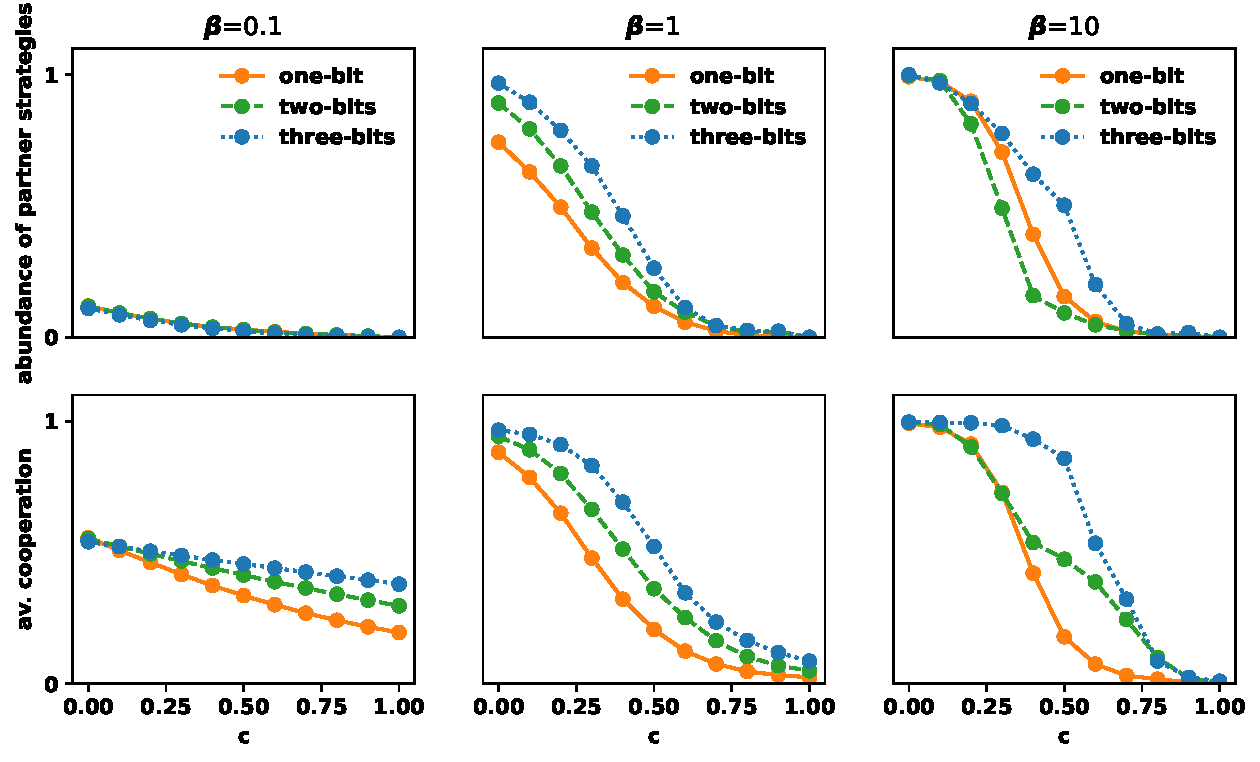
\includegraphics[width=\textwidth]{figures/abundance_of_partner_strategies.pdf}
  \caption{The abundance of partner strategies for $n=1,2,3$ and $b=1, c=0.5$.}
\end{figure}

\begin{figure}[!htbp]
  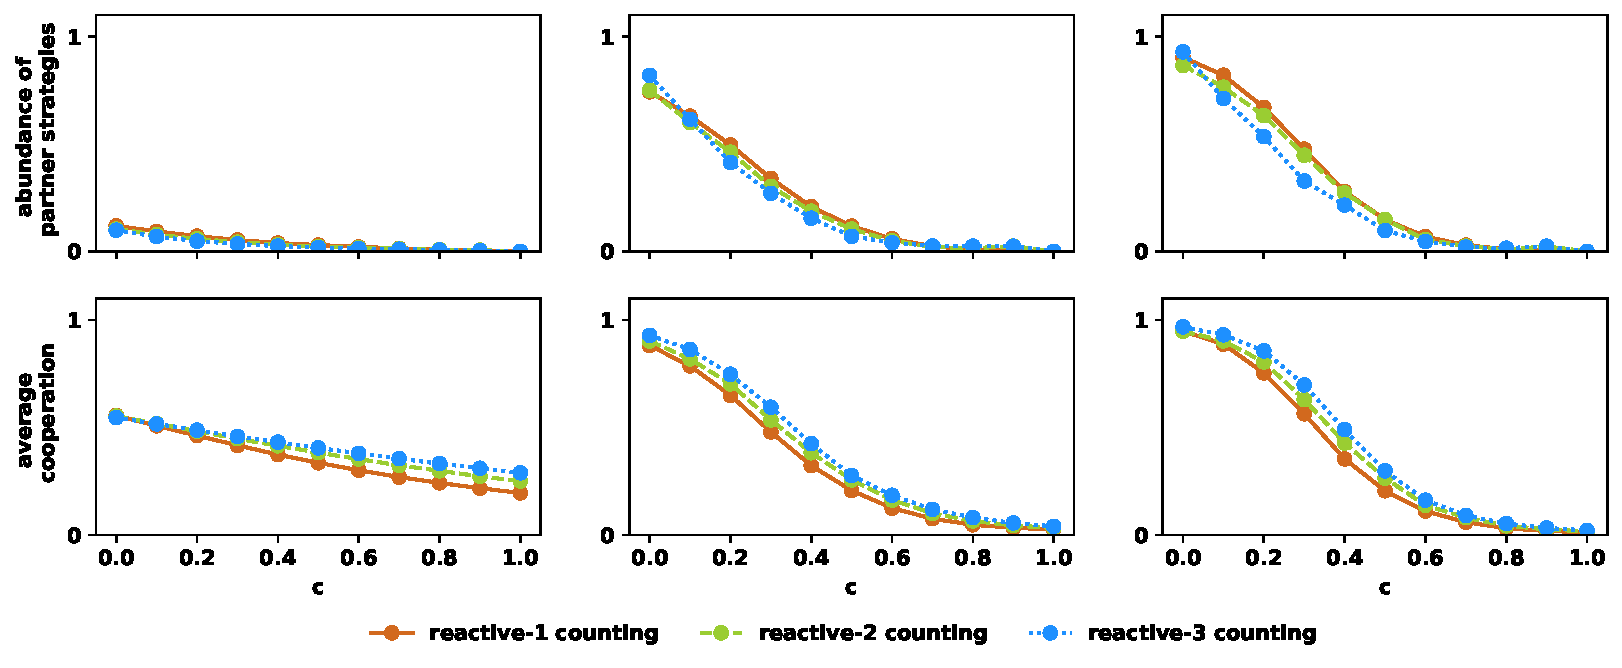
\includegraphics[width=\textwidth]{figures/abundance_of_partner_counting_strategies.pdf}
  \caption{The abundance of partner counting strategies for $n=1,2,3$ and $b=1, c=0.5$.}
\end{figure}

\begin{figure}[!htbp]
  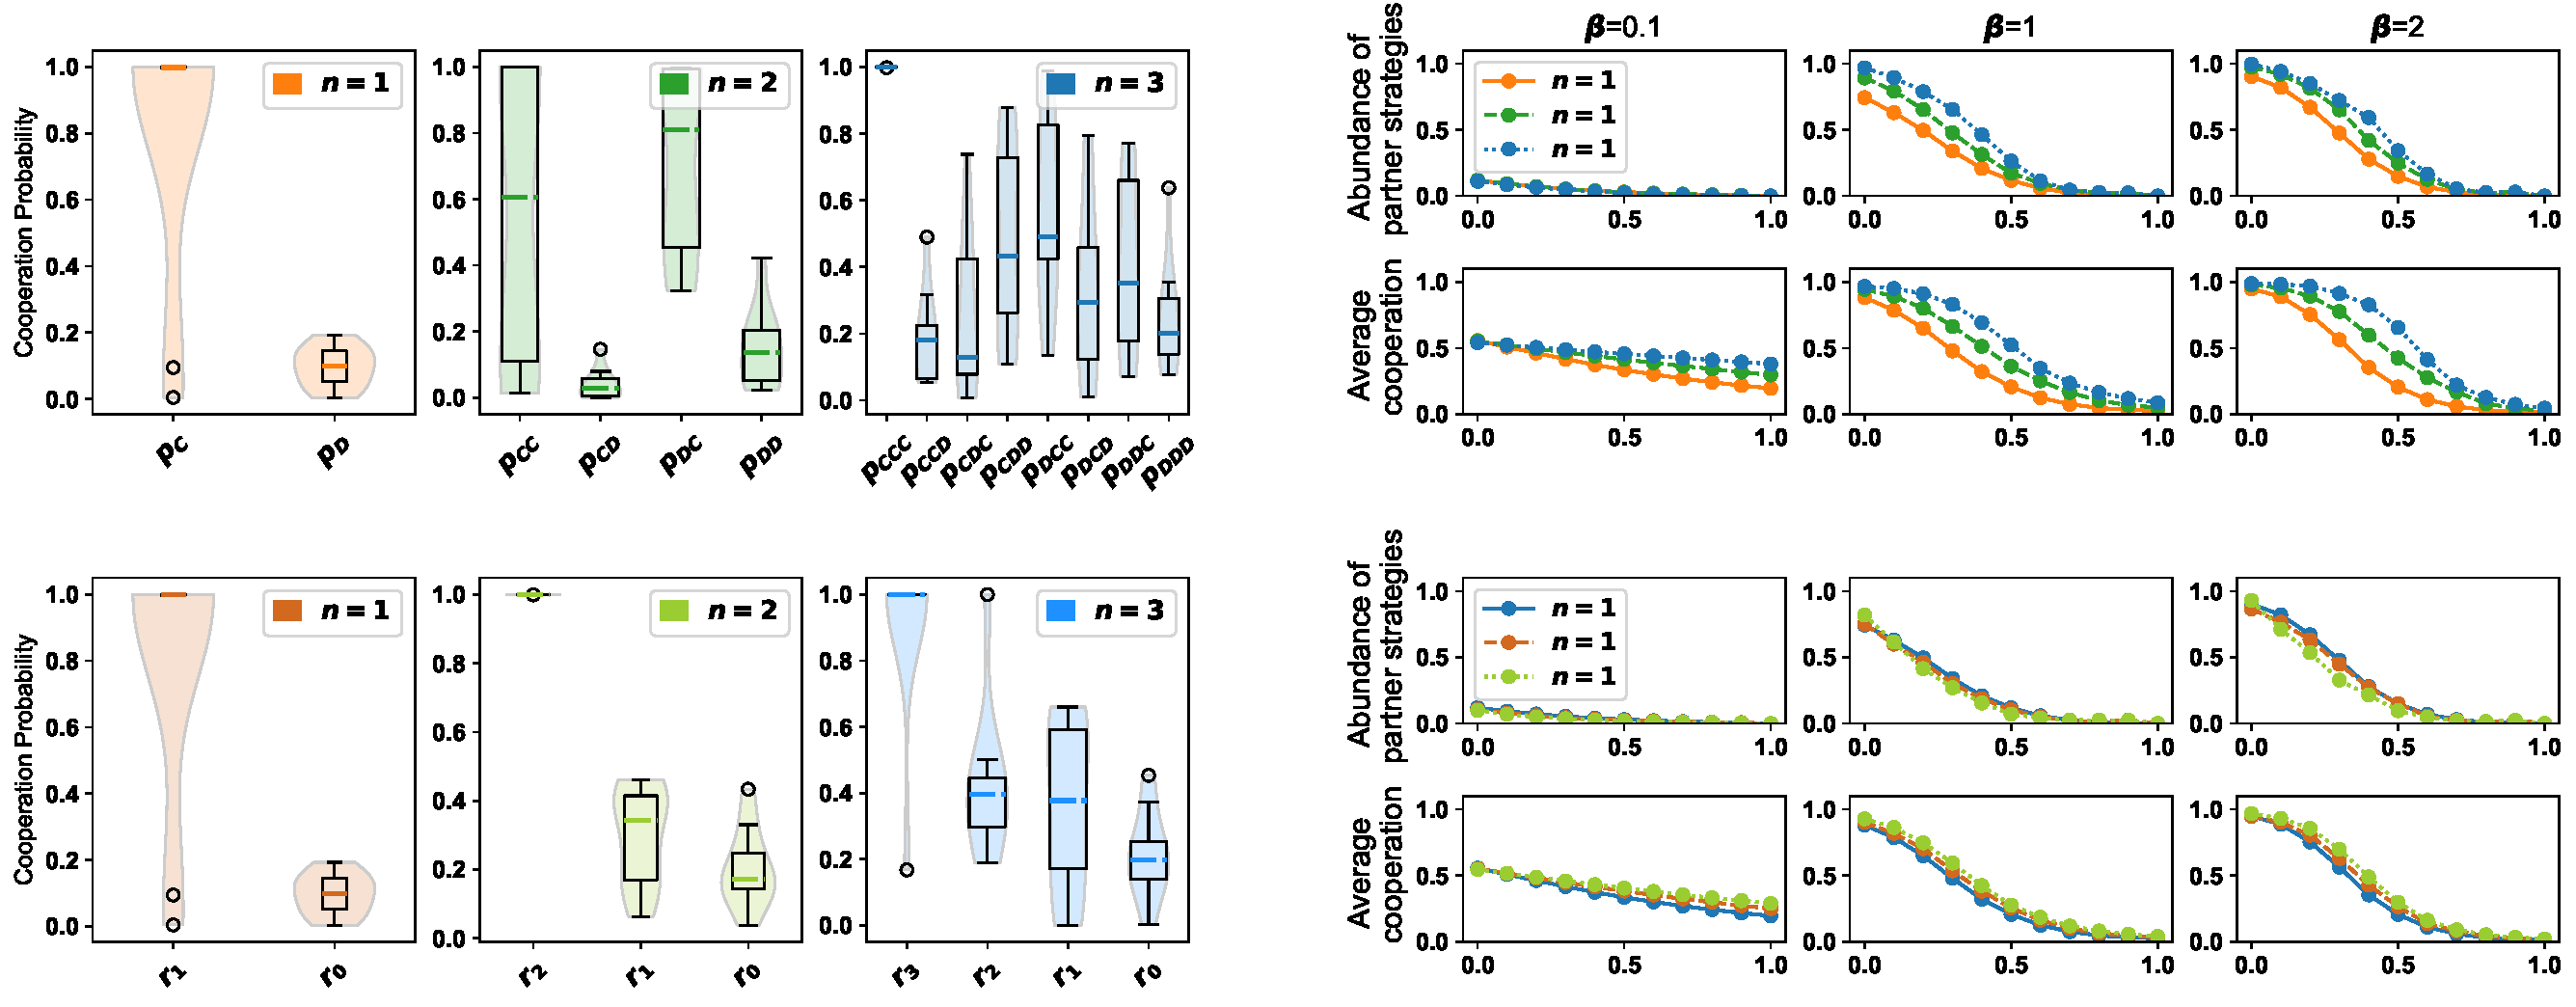
\includegraphics[width=\textwidth]{figures/abundant_strategies.pdf}
  \caption{The most abundant reactive-$n$ strategies for $n=1,2,3$ and $b=1, c=0.5, \beta=1$.}
\end{figure}

\begin{figure}[!htbp]
  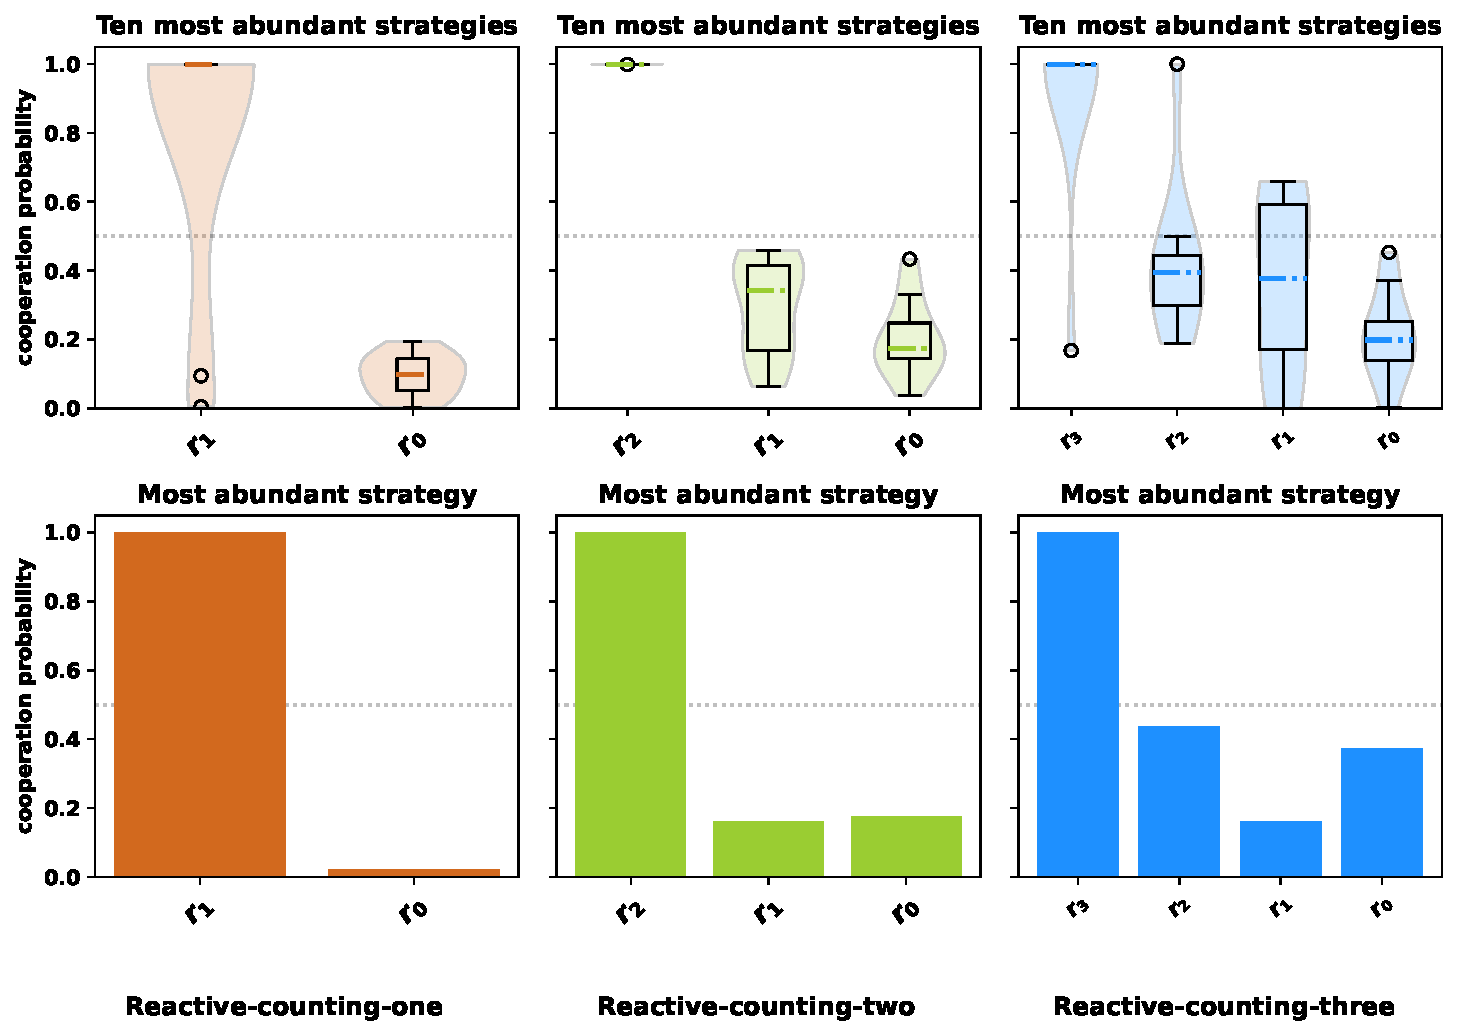
\includegraphics[width=\textwidth]{figures/abundant_strategies_counting.pdf}
  \caption{The most abundant reactive-counting-$n$ strategies for $n=1,2,3$ and $b=1, c=0.5, \beta=1$.}
\end{figure}

% \begin{figure}
%   \includegraphics[options]{fig}
% \end{figure}

~\\
\bibliography{bibliography.bib}

\end{document}